\section{Western Region Climate Data Analysis}

This analysis shows the temperature distribution across districts in the Western region of Nepal using spatial data visualization.

\subsection*{Filtering Districts}

\begin{verbatim}
# List of districts to match
district_list <- c("Gorkha", "Kaski", "Lamjung", "Manang", "Syangja",
                   "Arghakhanchi", "Gulmi",
                   "Nawalparasi", "Palpa", "Rupandehi", "Baglung",
                   "Myagdi", "Parbat","Mustang")

filtered_data_western <- df_climate[df_climate$District%in% district_list,]
\end{verbatim}

\subsection*{Geoplot for Temperature Distribution in Western Region}

\begin{verbatim}
# Calculate average temperature per district
plot_western <- filtered_data_western %>%
  group_by(District) %>%
  summarise(
    avg_temp = mean(Temp_2m, na.rm = TRUE),
    Latitude = first(Latitude),
    Longitude = first(Longitude)
  )

# Merge temperature data with spatial data
nepal_temp_west <- left_join(nepal_districts, plot_western , by = "District")

# GeoplotPlot
ggplot(data = nepal_temp_west) +
geom_sf(aes(data = avg_temp), color = "black") +
geom_point(aes(x = Longitude, y = Latitude, color = avg_temp), 
  size = 4) +  # Points for avg_temp
geom_text(data = plot_western, aes(
  x = Longitude, 
  y = Latitude, 
  label = District),
  size = 1.5, vjust = -0.5, color = "black") +
scale_color_gradient(low = "yellow", high = "red") +  # Color scale
labs(
  title = "Temperature Map of Nepal", fill = "Temperature"
  ) +
theme_minimal()
\end{verbatim}

% Figure here-----------------------------
\begin{figure}[h]
    \centering
    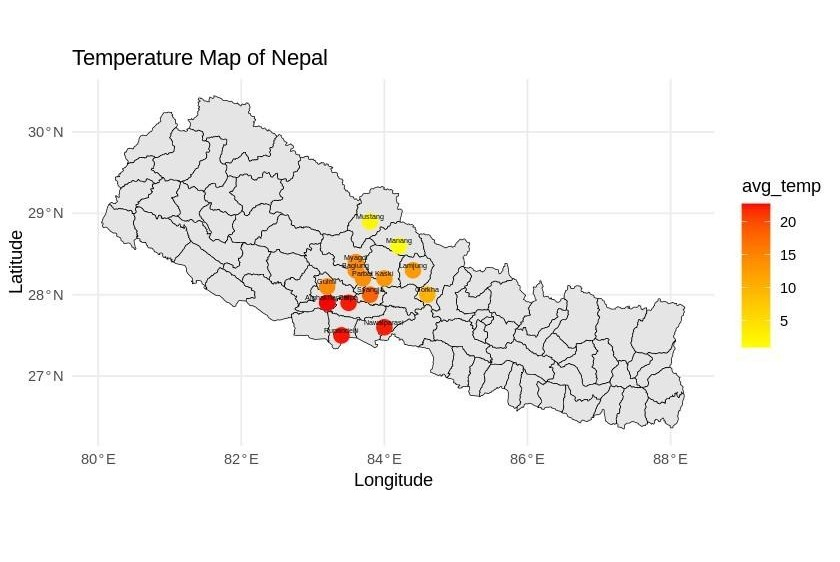
\includegraphics[width=0.6\textwidth]{figures/map_west.jpg}
    \caption{Temperature Map of Western Region}
\end{figure}

\subsection*{Scatter Plot of Temperature vs. Precipitation with Wind Speed by Season}

\begin{verbatim}
ggplot(filtered_data_western, aes(
  x = Temp_2m, 
  y = Precip, 
  color = Season, 
  size = WindSpeed_10m)) +
geom_point(alpha = 0.7) +
scale_color_manual(values = c(
    "Spring" = adjustcolor("yellow", alpha.f = 0.6),
    "Summer" = adjustcolor("red", alpha.f = 0.6),
    "Fall" = adjustcolor("orange", alpha.f = 0.6),
    "Winter" = adjustcolor("blue", alpha.f = 0.6)
  )) +
scale_size_continuous(range = c(1, 10)) +
labs(
title = "Scatter Plot of Temperature vs. Precipitation with Wind Speed Size",
x = "Temperature (°C)",
y = "Precipitation (mm/day)",
color = "Season",
size = "Wind Speed (10m)"
) +

theme_minimal()
\end{verbatim}

% Figure here-----------------------------
\begin{figure}[h]
    \centering
    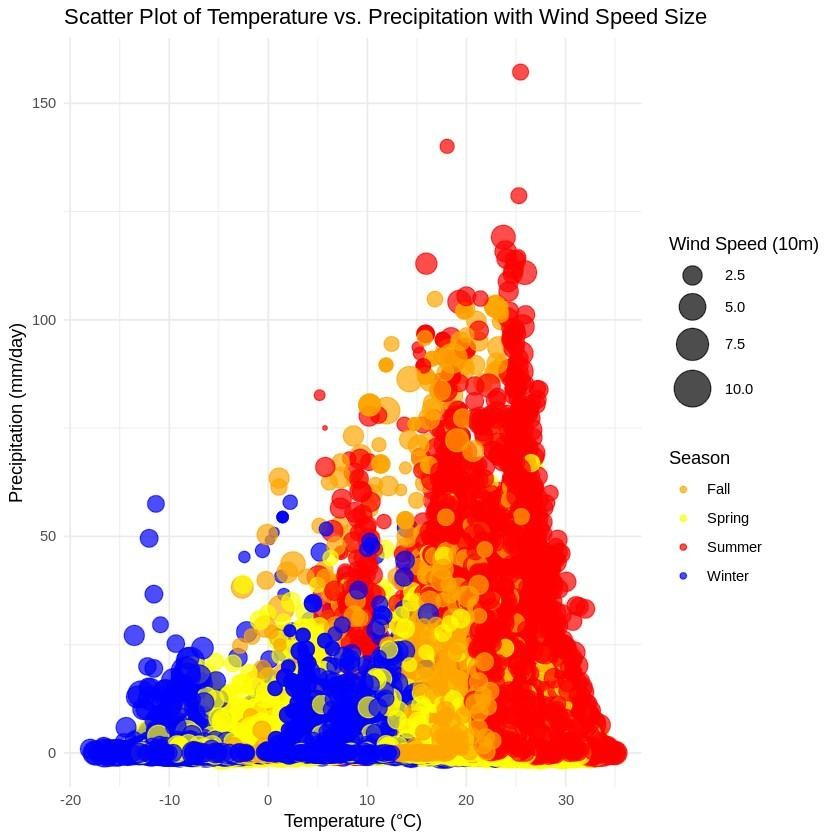
\includegraphics[width=0.5\textwidth]{figures/scatter_west.jpg}
    \caption{Scatterplot showing Temperature vs. Precipitation with Wind Speed by Season}
    \label{fig:scatter_temp_precip_wind}
\end{figure}

\subsection*{Histogram of Wind Speed with Density Curve for Western Region}

\begin{verbatim}
ggplot(filtered_data_western, aes(x = WindSpeed_10m)) +
geom_histogram(aes(y = ..density..), bins = 30, fill = "skyblue", 
color = "black", alpha = 0.7) + 
geom_density(color = "blue", linewidth = 1) + 
labs(
title = "Histogram of Wind Speed with Density Trendline for Western Region",
x = "Wind Speed (10m)",
y = "Density") +
theme_minimal()
\end{verbatim}

% Figure here-----------------------------
\begin{figure}[h]
    \centering
    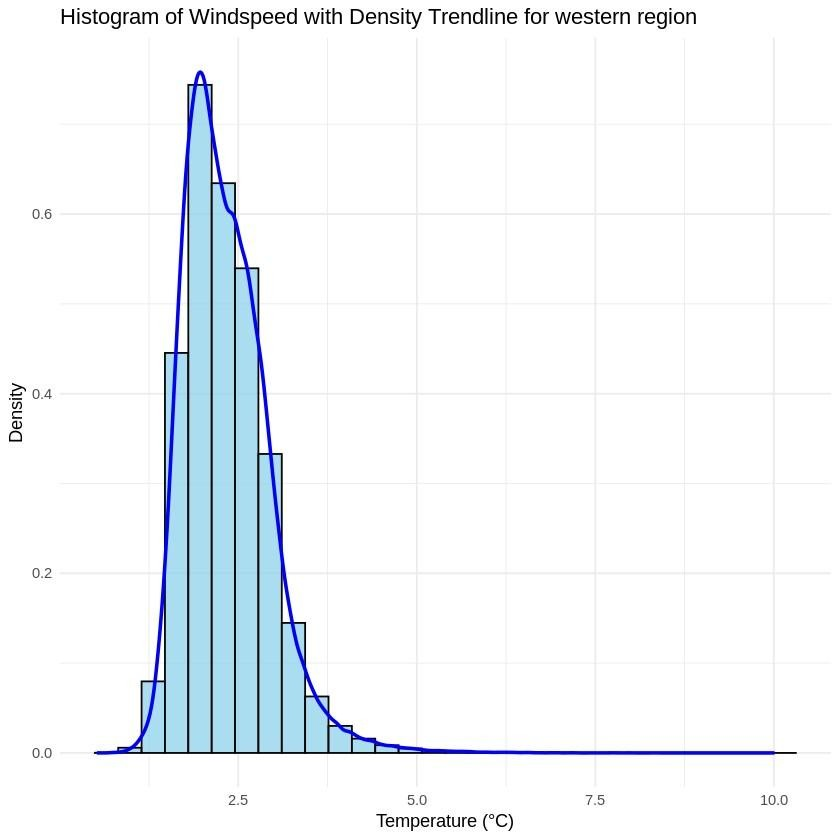
\includegraphics[width=0.5\textwidth]{figures/hist_west.jpg}
    \caption{Histogram of Wind Speed with Density Trendline for Western Region}
\end{figure}

\subsection*{Precipitation Trend Over Time in Western Region}

\begin{verbatim}
ggplot(filtered_data_western, 
aes(
  x = Date, 
  y = Precip)) +
geom_line(color = "blue") +
labs(
  title = "Precipitation Trend Over Time - Western Region",
  x = "Date", 
  y = "Precipitation (mm)") +

  theme_minimal()
\end{verbatim}

% Figure here--------------------------
\begin{figure}[h]
    \centering
    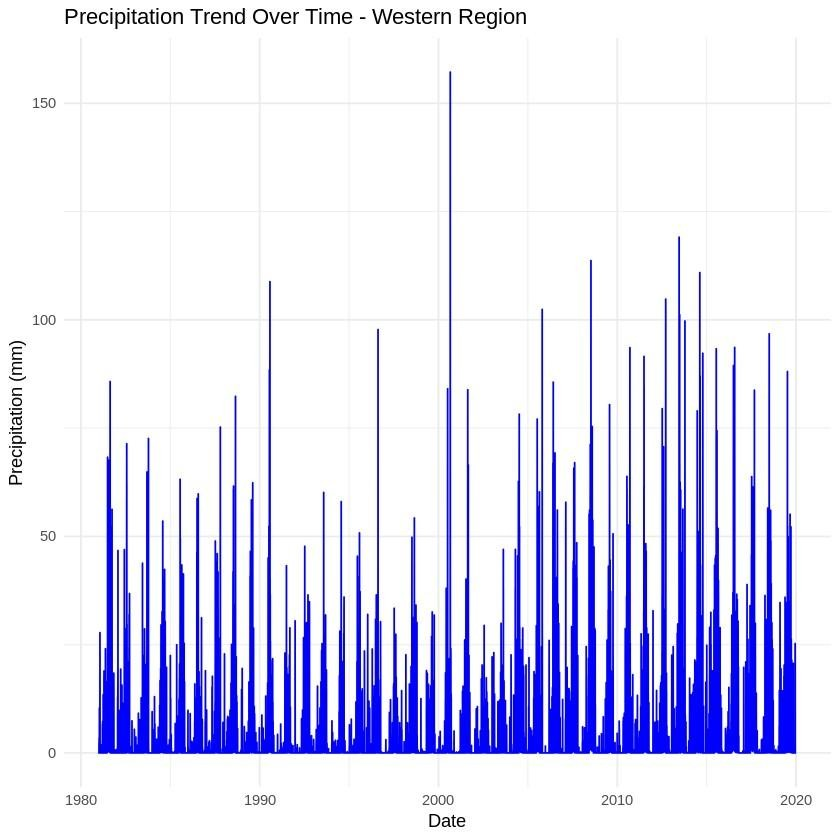
\includegraphics[width=0.5\textwidth]{figures/precip_west.jpg}
    \caption{Precipitation Trend Over Time - Western Region}
\end{figure}

\subsection*{Temperature Distribution by Season}

\begin{verbatim}
ggplot(filtered_data_western, aes(x = Season, y = Temp_2m, fill = Season)) +
  geom_boxplot() +
  labs(title = "Temperature Distribution by Season",
       x = "Season", y = "Temperature (°C)") +
  theme_minimal() +
  theme(legend.position = "none")
\end{verbatim}

% Figure here-----------------------------
\begin{figure}[h]
    \centering
    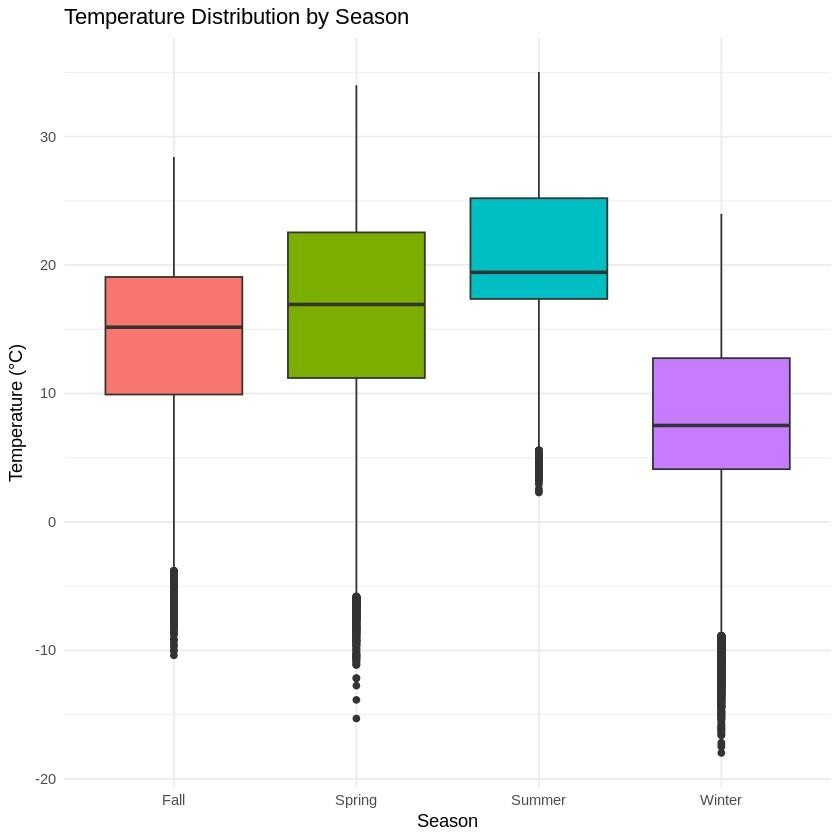
\includegraphics[width=0.5\textwidth]{figures/box_west.jpg}
    \caption{Temperature Distribution by Season in Western Region}
\end{figure}
